\subsection{Cambios realizados sobre la segunda entrega}

En el modelo entidad/relación, se elimina el atributo ``Género relacionados'' de la entidad ``Autor'' y se añade una relación entre esta entidad y la entidad ``Género''. Además, se añade una relación de herencia entre ``Usuario'' y ``Usuario con privilegios''. También se eliminan las relaciones ``Añadir'', ``Modificar'' y ``Borrar'', ya que solo serían necesarias si quisiéramos almacenar qué usuario almacena, modifica o borra una canción determinada. Consideramos que esta información no es propia de nuestro sistema y por la complejidad que implica, decidimos eliminarlas.

\subsection{Diseño lógico}

El siguiente diagrama es el paso a tablas de nuestro modelo entidad/relación disponible en el apartado anterior.

\begin{figure}[H]
  \centering
  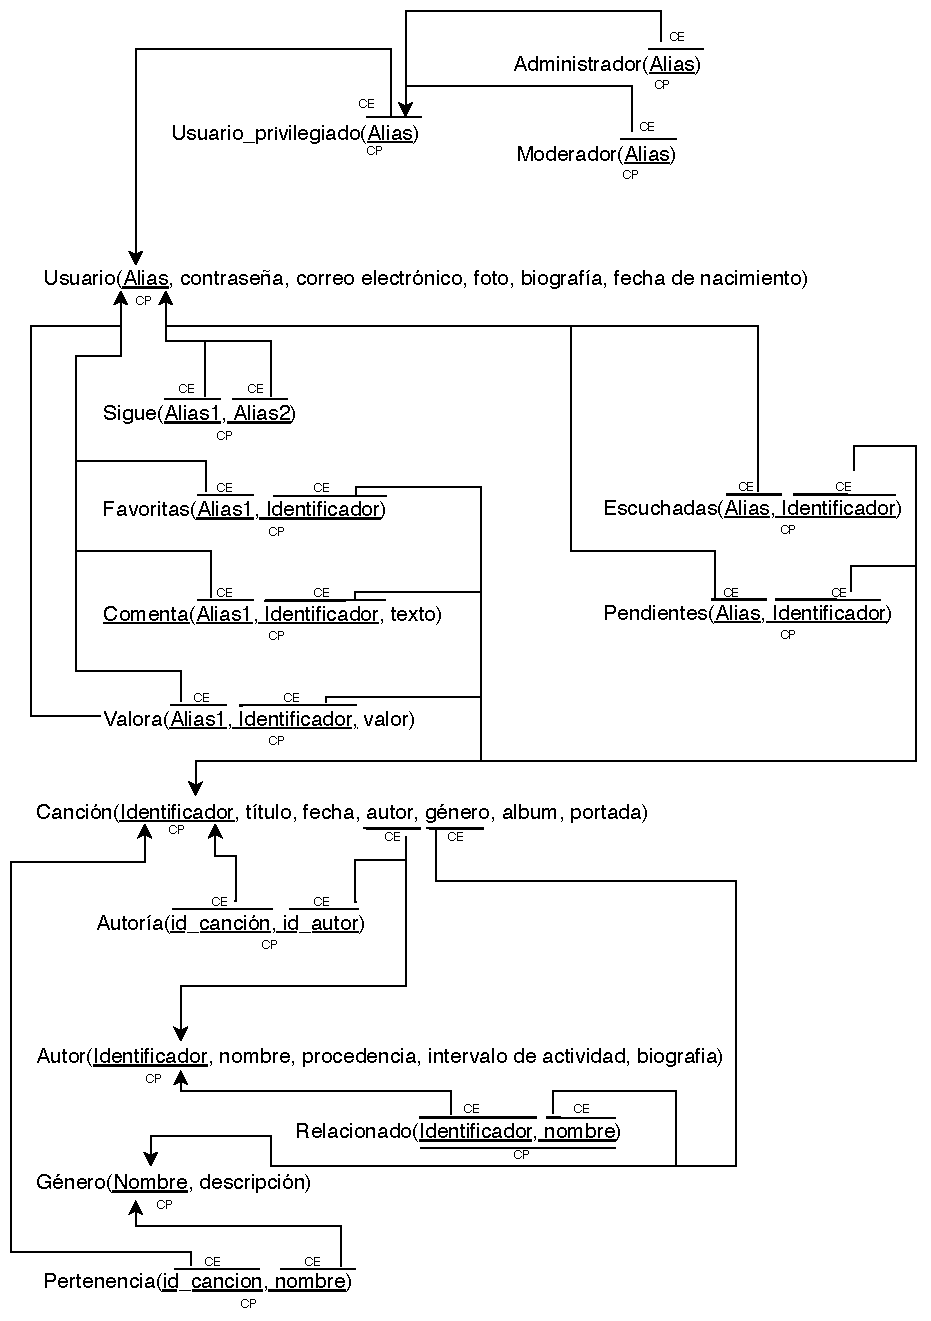
\includegraphics[scale=0.9]{diagramas/paso_a_tablas.pdf}
\end{figure}

\subsection{Diseño físico}

A continuación se exponen las secuencias SQL necesarias para la creación de todas las tablas del sistema.

\lstinputlisting[language=SQL]{src/ddsi.sql} 

\subsection{Funcionalidad a nivel de base de datos}

A continuación se exponen los disparadores creados por cada uno de los integrantes del grupo.

\subsubsection{Subsistema de música}

El primer trigger comprueba que la canción añadida tiene como autor y género uno de los existentes, RS \ref{rsu:aniadir-cancion}. El segundo, que la fecha de comienzo de actividad de un autor es anterior al presente, RS \ref{rsu:aniadir-autor}.

\lstinputlisting[language=SQL, firstline=1, lastline=18]{src/trigger.sql} 
\lstinputlisting[language=SQL, firstline=51, lastline=63]{src/trigger.sql}

\subsubsection{Subsistema de usuarios}

El disparador de usuario comprueba que al insertar un usuario en la base de datos, el formato del campo ``correo electronico'' sea correcto.
\lstinputlisting[language=SQL, firstline=20, lastline=30]{src/trigger.sql} 

\subsubsection{Subsistema social}
El disparador del subsistema social comprueba que antes de dejar un comentario en una canción el usuario la haya escuchado, RS 4.1.
\lstinputlisting[language=SQL, firstline=32, lastline=49]{src/trigger.sql} 
